\documentclass[12pt, letterpaper, titlepage]{article}

\usepackage{amsmath, amsfonts}
\usepackage{booktabs}
\usepackage{amsthm}
\usepackage{graphicx}
\usepackage[margin=1in]{geometry}
\usepackage{hyperref}
\usepackage{cleveref}
\hypersetup{colorlinks = true, linkcolor = blue, citecolor=blue, urlcolor = blue}
\usepackage{natbib}
\usepackage{float}
\usepackage{setspace}
\usepackage{pdfpages}
\usepackage[pagewise]{lineno}
\usepackage{mwe}
\usepackage{comment}
\linenumbers*[1]
% %% patches to make lineno work better with amsmath
\newcommand*\patchAmsMathEnvironmentForLineno[1]{%
 \expandafter\let\csname old#1\expandafter\endcsname\csname #1\endcsname
 \expandafter\let\csname oldend#1\expandafter\endcsname\csname end#1\endcsname
 \renewenvironment{#1}%
 {\linenomath\csname old#1\endcsname}%
 {\csname oldend#1\endcsname\endlinenomath}}%
\newcommand*\patchBothAmsMathEnvironmentsForLineno[1]{%
 \patchAmsMathEnvironmentForLineno{#1}%
 \patchAmsMathEnvironmentForLineno{#1*}}%

\AtBeginDocument{%
 \patchBothAmsMathEnvironmentsForLineno{equation}%
 \patchBothAmsMathEnvironmentsForLineno{align}%
 \patchBothAmsMathEnvironmentsForLineno{flalign}%
 \patchBothAmsMathEnvironmentsForLineno{alignat}%
 \patchBothAmsMathEnvironmentsForLineno{gather}%
 \patchBothAmsMathEnvironmentsForLineno{multline}%
}

% control floats
\renewcommand\floatpagefraction{.9}
\renewcommand\topfraction{.9}
\renewcommand\bottomfraction{.9}
\renewcommand\textfraction{.1}
\setcounter{totalnumber}{50}
\setcounter{topnumber}{50}
\setcounter{bottomnumber}{50}

\newcommand{\jy}[1]{\textcolor{blue}{JY: #1}}
\newcommand{\eds}[1]{\textcolor{red}{EDS: (#1)}}
\newcommand{\of}[1]{\textcolor{violet}{OF: #1}}


\title{On Devon Allen's Disqualification at the 2022 World Track and Field 
Championships} 

\author{Owen Fiore\\
%   \href{mailto:owen.fiore@uconn.edu}
% {\nolinkurl{owen.fiore@uconn.edu}}\\
  Elizabeth D. Schifano\\
  Jun Yan\\[1ex]
  Department of Statistics, University of Connecticut\\
}
\date{}

\begin{document}
\maketitle

%Abstract should be 200 words
%Devon Allen was disqualified in 2022... discussions about dq, talk methods and 
%models, venue effect, and conclusion
\begin{abstract}
Devon Allen was disqualified in the men's 110 meter hurdle final of the 2022
World Track and Field Championships after registering a reaction time of 0.099 
seconds, 0.001 seconds faster than what is allowed. Following the games, 
bloggers on the running website LetsRun concluded that the reaction times  
from the 2022 World Championships seemed to be generally faster compared to the 
other reaction times they considered, but they did not perform any formal 
statistical analysis. This paper questions if athletes who competed at the 2022
World Track and Field Championship had similar times at other competitions and
if 0.1 seconds is a reasonable disqualification barrier. To do so, we employ a 
signed-rank test for clustered data to compare reaction times for the same 
athletes at different competitions and a generalized linear mixed model 
with random venue (year) effect and a random heat effect within venue 
in order to model the reaction time data. This matter needs to be addressed 
because disqualification based on allowable reaction time will continue to be an
issue in future world championships.


\bigskip\noindent{\sc Keywords}:
False Start, Hurdles, Reaction Time, Seiko 

\end{abstract}

\doublespace


\section{Introduction}
\label{sec:intro}


Devon Allen, an alumnus of the University of Oregon in Eugene, Oregon, was
expected to be a contender for the 2022 World Track and Field Championships 110 
meter hurdle. After running the event in 12.84 seconds in early June 2022 
(only 0.04 seconds away from the world record \citep{wa2022preview}) and coming 
in third at the United States Track and Field Championships also in Eugene 
in late June, Allen was poised to compete in the 2022 World Track and 
Field Championships in August, which would also be held in Eugene, Oregon.
At the World Championships, Allen made it through the preliminary
heats and semifinals to reach the final heat while posting reaction times of 
0.123 and 0.101 in his preliminary heat and semifinal, respectively. 
His disqualification in the final heat by reacting in 0.099 seconds, just 0.001
seconds faster than the 0.1 threshold set by the International Association of
Athletics Federations (IAAF), was met
with shock from both Allen and fans alike. NBC, who was broadcasting the
championships in the United States, later uploaded a video to their YouTube
channel that showed the disqualification
(\url{https://www.youtube.com/watch?v=D6NXTMo-1yM}).
The crowd erupted with jeers
when they realized that Allen was disqualified, angry at the result. Had Allen 
reacted just 0.001 seconds slower he would have been allowed to compete.


Allen's disqualification has been discussed extensively in online communities
such as \url{www.LetsRun.com}, a website that is part message board and part
news. The message board,
which functions similarly to Reddit, is very active during important running
events, including during the finals of major events such as
the Olympics and the World Track and Field Championships. However, it is the
news section of the website that generated articles such as \citet{johnson2022data}
and \citet{johnson2022was} from  Robert Johnson, who created and runs 
the LetsRun website. He argued that there was an error
with the timing equipment at the 2022 World Track and Field Championships and
cited graphs, computed descriptive statistics such as median reaction times, and 
compared the reaction times at the 2022 World Track and Field Championships to 
other competitions
such as the United States Track and Field Championships and other World Championships.
The comparisons lacked formal statistical analysis, however. 
The alleged 99.95\% chance Allen was wronged 
came from Johnson claiming there is a $(1/13)^3$ chance that the fastest 
reaction times over the past 13 competitions of the men's 100 meter, men's 110 
meter hurdle, and women's 100 meter would all come from the same year 
\citep{johnson2022was}.


Reaction time in sprint and hurdle events has been studied by many authors.
\citet{pain2007sprint} examined reaction times for nine male athletes. The
fastest athlete of the nine had, on average (even with their two fastest times 
removed), a reaction time of 0.087 seconds and a standard deviation of 0.004
seconds. Two other athletes were able to react similarly when under certain
muscular tightening conditions \citep{pain2007sprint}. 
In a study commissioned by IAAF,
\citet{komi2009iaaf} recommended that the disqualification 
barrier be decreased to allow sprinters to
react faster, and suggested 0.08 or 0.085 seconds as possible new thresholds.
Unfortunately, IAAF has not changed the reaction barrier since it was
implemented at the 1999 World Track and Field Championships.
It is unknown how many athletes since the 2009 study could have potentially
benefited from this, but it is probable that there are others besides Allen who
could have. Additionally,
\citet{komi2009iaaf} recommended that high speed cameras be used to
change the reaction time criteria from pushing off on the block to body
movement. This could provide a more accurate representation of reaction time, 
and thus the possibility of a false disqualification would be lowered.
The possibility of using a video-based medium has been shown to be a reliable
measure of reaction time \citep{mudric2015evaluation}.


\citet{pilianidis2012start} found
significant differences between reaction times at several world championships
between 1997 and 2009 for the men's 110 meter hurdles. Another important
conclusion was that reaction times did not decrease over the twelve years
covered by the research in the study \citep{pilianidis2012start}. This 
contradicts the results of \citet{zhang2021correlation}, which indicated that 
year of competition has a significant effect on reaction times. Their
analysis looked at data from the 2011-2019 World Championships across multiple
sprint events and concluded that from 2011 to 2019, reaction times got
faster. However, not all studies have been in favor of a decrease in the
reaction time barrier. \citet*{brosnan2017effects} argue for increasing 
the reaction time barrier to 0.115 seconds, and cited evidence from European 
Championships and World Championships in their article. A study looking 
at the 2008 Olympics likewise supported the conclusion that athletes could not
react in as little as 0.1 seconds \citep{lipps2011implications}. Another study
concluded that visual reaction times to the starting gun may be faster by 0.007
seconds than the IAAF method, which is from force on block starts 
\citep{holmes2018method}. While this may seem trivial, Allen was disqualified
only by 0.001 seconds. It is also worth noting that one study looking at data 
from various IAAF meets found that the fastest reaction times for men occurred 
between the ages of 26 and 29 \citep{tonnessen2013reaction}. This is notable 
because Allen was 27 years old at the 2022 World Track and Field Championships 
and likely at his physical peak.


The objective to this paper is to analyze the reaction times at the 2022 World 
Track and Field Championships to check for any abnormalities, and we approach
this in two different ways. First we compare reaction times for athletes who 
have competed at additional competitions to the 2022 World Track and Field 
Championship. By comparing reaction times from the same athlete across multiple
competitions we are able to determine if the 2022 reaction times differed 
significantly from those of other competitions. Then we look at a longer time horizon
and model the reaction times of every non-disqualification since the 1999 World 
Championships, using a gamma linear mixed-effects model with two random effects: 
one effect for the year and a second effect for the heat nested within each year.
Based on the fitted model, we can then estimate the probability of a reaction 
time being below a certain threshold (e.g., 0.1). 
Our investigation into reaction times is important not only because of its
implications for future races, but also because reaction times have
been shown to affect the overall time of the race \citep{delalija2008reaction}.
Thus, faster reaction times lead to faster overall times, which is the goal of
every sprinter who steps onto the track.


The rest of this paper is organized as follows. Section~\ref{sec:Data} details 
how the two types of data were collected, as the signed-rank test as described
in Section~\ref{sec:rank} uses slightly different data than the generalized 
linear mixed-effect model (GLMM) that is further developed in 
Section~\ref{sec:glmm}. Section~\ref{sec:Results} provides the results of the two
analyses and ends by questioning the reaction time barrier. Lastly, 
Section~\ref{sec:concludingremarks} discusses the impact and limitations of the
paper. All the data and code of our analysis are available in a supplement.


\section{Data} \label{sec:Data}

There are two types of data that are explored throughout this paper. For the
signed-rank tests described in Section~\ref{sec:rank}, the data comes from 
athletes who competed in the 2022 World Championships and another competition 
(2019 World Championships, 2023 World Championships, or 2022 national 
championships). For the GLMM described in Section~\ref{sec:glmm}, data comes
from every world championships from 1999 to 2023. This investigation started 
shortly after the 2022 World Championships, but as the 2023 data has now become 
available, we are pleased to include it in both of our analyses, and it did not
significantly change our results \citep{WAData}. 


\subsection{Comparison Data with 2022 World Championships}
\label{sec:databeyond}

The motivation for looking beyond World Championships data came from an 
exploratory analysis examining how United States athletes reacted at the 
2022 United States Track and Field Championships.


\subsubsection{2022 National Competitions}\label{sec:datanational}
From June 23-26, 2022, the United States held its Track and Field Championships 
at Hayward Field in Eugene, Oregon to decide who to send to the World 
Championships being held at the same venue in August. Thus, we can establish a 
baseline for the four United States athletes who competed in at least one round 
of both events: Trey Cunningham, Daniel Roberts, Grant Holloway, and Devon Allen.  
Every athlete reacted faster in all the World Track and Field Championships 
races compared to the United States Track and Field Championships races. The 
dataset of the four United States athletes is too small to perform any 
meaningful statistical analysis, but the data was expanded to include reaction 
times for 11 more athletes who competed at other national competitions (many of which were 
held from May-July of 2022). This data was difficult to find, as the data is not
centrally located but instead found on different national websites (often 
recorded in the national language without translation).


Each athlete was designated as a ``cluster'' and the stage of competition (national
or international) was specified for each competition within the cluster (athlete).
Thus, this is subunit level grouping where we assign the treatment, national or
international, within each cluster. Cluster sizes range from three to six, with
one cluster of size three, six clusters of size four, two clusters of size five,
and two clusters of size six. We chose to include preliminary rounds in this
section as well as in Section~\ref{sec:data2019} in order to increase the size 
of our data. Without data from the preliminary rounds, the number of observations
dropped from 65 to 26 and the number of athletes included in the analysis
decreased from 15 to 9.


\subsubsection{Other World Track and Field Championships}\label{sec:data2019}
The 2019 and 2023 World Track and Field Championships data is included in the 
larger dataset described in Section~\ref{sec:dataworld}, but we can also use it
similarly to how we used national level in Section~\ref{sec:datanational}. We
can compare the times of athletes who participated in the 2022 Championships with
their times at another World Championships: 2019 and/or 2023.


While it is theoretically possible that athletes got faster 
between 2019 and 2022 or 2022 and 2023, it is important to 
remember that these are some of the fastest sprinters on the planet, and thus
improving on elite times is not easy. Once again we repeat a similar procedure
as in Section~\ref{sec:datanational}; we assign each athlete to be a cluster and
within each cluster label times to be from either the 2019, 2022, or 2023 World
Championships. When comparing 2019 and 2022 we look at data from 15
athletes, with two clusters of size two, three clusters of size three, five 
clusters of size four, two clusters of size five, and three clusters of size six.
When comparing 2022 and 2023 we look at data from 22 athletes, with seven 
clusters of size two, three clusters of size three, six clusters of size four,
and six clusters of size five.

\begin{figure}[tbp]
  \centering
  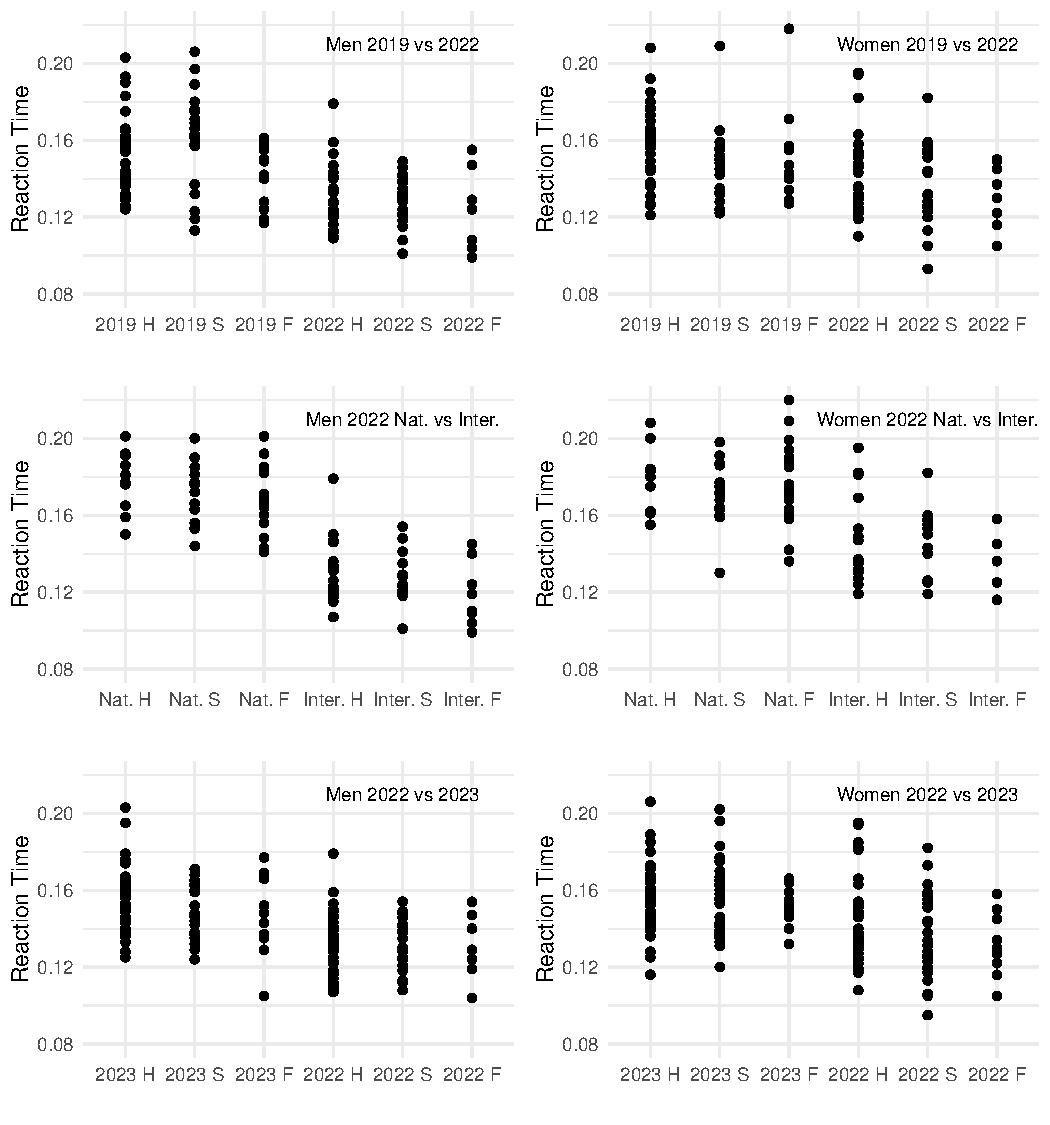
\includegraphics{RankScatterPlots}
  \caption{The top graph shows the reaction times of athletes who competed at 
	least once each at the 2019 and 2022 World Championships. The middle graph 
	shows the reaction times of athletes who competed at least once each at the 
	2022 and 2023 World Championships. The bottom graph shows the reaction times 
	of athletes who competed at least once at their country's
        2022 national championships and the 2022 World Championships.}
  \label{fig:RankScatterplots}
\end{figure}


Figure~\ref{fig:RankScatterplots} shows the data that will be analyzed
with the rank-based methods (described in Section~\ref{sec:rank} with results in 
Section~\ref{subsec:Results_Rank}). In each of the three graphs, the reaction 
times for athletes who competed at the 2022 World Championships
are compared to their reaction times at another at which they competed. 
It is worth noting that each instance of the 2022 data is different, because
those who competed at both the 2019 and 2022 World Championships will be
different athletes than those who competed at both the 2022 and 2023 World
Championships. This data was only for athletes who competed
in at least one race at each championship, however it is possible for athletes
to have competed in one race in 2019 and two races in 2022.
%The 2022 World
%Championship Heats and Semifinals both had on average lower reaction times than
%their respective 2019 races, and the 2022 finals were substantially faster. 
The 2022 World
Championship Heats and Semifinals both had on average lower reaction times than
their respective other (2019, 2023 or 2022 national) races, and the 2022 World 
Championship finals were substantially faster. 
\eds{please check change}
It
is also worth noting is that the fastest reaction time in the 2022 World
Championships Finals and Semifinals both came from Devon Allen, but the 
difference between 0.101 and 0.099
seconds was the difference in what caused him to be disqualified. 


\subsection{World Championships 1999--2023}\label{sec:dataworld}


Data was taken from the World Athletics 
and covers the men's 110 meter hurdles from 1999 to 2023.
We focus on the reaction times during the 
semifinal and final heats only, as reaction times from preliminary heats are 
often not as fast as those in later heats \citep[e.g.,][]{zhang2021correlation}. 
For analysis purposes, we will pool reaction times of men's final and 
men's semifinal heats together which increases the sample size. This is 
advantageous because in some years there are very few finals observations, such
as in 2022, when there were only five data points due to two disqualifications 
and one athlete who did not compete. This is the data that we will reference
throughout the rest of the paper unless otherwise noted. We also consider data 
that excludes 2022 to see how our analysis differs based on the exclusion of one
particular year of interest.


The data under consideration is summarized using side-by-side boxplots in 
Figure~\ref{fig:Boxplot}. It is clear that the reaction times in the 2022
boxplot are lower (indicating faster reaction times) than in many of the other
years. The median reaction time in 2022 was 0.129 seconds,  compared to 0.156
seconds, which is what \citet{brosnan2017effects} found when looking at data
from 1999 to 2014. We can also see from Figure~\ref{fig:Boxplot} that the 
reaction times clearly differ from year to year. The venue of the World 
Championships changes each year, so weather or climate related factors such as 
humidity, precipitation, elevation, may indeed play a role, but additionally,
both the technology and false start penalization rules have changed over the 
study period.


\begin{figure}[tbp]
  \centering
  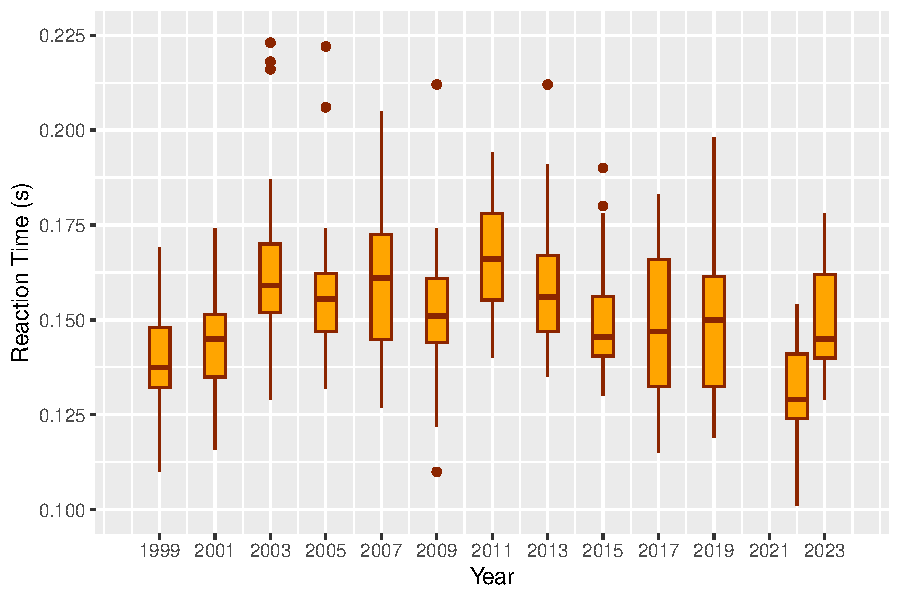
\includegraphics{Boxplot}
  \caption{The reaction times from 1999 to 2023 for the men's 110 meter hurdle.}
  \label{fig:Boxplot}
\end{figure}


From 2007 to 2009, the IAAF (the former name for World Athletics, and the 
governing body for the World Track and Field Championships) instituted a rule 
change that allowed one warning false start before a sprinter was disqualified 
\citep{iaaf2009falsestart}. There were 18 male and 7 female false starts at the 
2007 World Championships, and 18 male and 7 female false starts at the 2009 World 
Championships. Starting in 2011, the rule was scrapped, and the old policy which
automatically disqualifies runners who false start was reinstated. This was 
desirable for World Athletics as false starts can make already lengthy track 
meets more tedious, both for athletes and viewers watching the television 
broadcast. By returning to the harsher policy and cracking down on false starts,
World Athletics had reduced men's false starts by two thirds in 2011 (6 male and
4 female disqualifications) \citep{iaaf2009falsestart}. \citet{haugen2013effect}
examined the effect of different false start rules that IAAF has imposed from 
1997 to 2009 and found statistically significant improvement in reaction times 
under more lenient rules.



\section{Methods} \label{sec:Methods}

The data described in Sections~\ref{sec:databeyond} and~\ref{sec:dataworld} were
analyzed with rank-based methods and a GLMM, respectively.


\subsection{Rank-based Comparison}\label{sec:rank}


To test the conjecture that the 2022 World Championships timing device may have 
led to faster recorded reaction times, we compare the reaction times of the same
athletes who have attended both the 2022 World Championships and other 
competitions. 
In this setting, we have clustered data with subunit grouping. In particular,
each athlete is a cluster and the multiple reaction times from the same athlete
can be from either the 2022 World Championships or otherwise.
Let $X_{ij}$ be the $j$th reaction time of athlete~$i$, $i = 1, \ldots, n$,
$j = 1, \ldots, m_i$ where $m_i$ is the number of observations from
athlete~$i$. Let $\delta_{ij}$ be the group indicator of $X_{ij}$; $\delta_{ij}
= 1$ if $X_{ij}$ is in group~1 (2022 World Championships) and $\delta_{ij} = 0$ 
otherwise. Athletes are
assumed to be independent, while subunit observations from the same athlete are
not. The null hypothesis $H_0$ to be tested is that there is no difference
between the two groups; i.e., the distribution of $X_{ij}$ remains the same
regardless of the group indicator $\delta_{ij}$.


\citet{datta2005rank} proposed an extension of the Wilcoxon rank-sum test to
clustered data with subunit-level grouping. The test is designed based on a
within-cluster resampling principle. Consider randomly picking one observation
from each cluster to form a pseudo-sample. Let $X_i^*$ be a random pick from the
$i$th cluster in the pseudo-sample and $\delta_i^*$ its group indicator. The
Wilcoxon rank-sum statistic for the pseudo-sample is
\[
W^* = \frac{1}{n + 1} + \sum_{i=1}^{n} \delta_{i}^{*} R_{i}^{*},
\]
where $R_{i}^{*}$ is the rank of $X_{i}^{*}$ in the pseudo-sample.
The test statistic $S$ is the average of $W^*$ averaged over all possible
pseudo-samples conditioning on the observed data and group indicators.
The mean and variance of $S$ under $H_0$ can be derived so that $S$ can be
standardized to form a $Z$ statistic which follows a standard normal distribution
asymptotically \citep[p.910]{datta2005rank}.


With our small sample size, the asymptotic normal distribution may not be
reliable, so we also use 1~million random permutations to simulate the null 
distribution of the test statistic.
This method is available from the \texttt{clusWilcox.test()} function
with \texttt{method = `ds'} (for \underline{D}atta and \underline{S}atten) and 
\texttt{exact = TRUE} from R package
\texttt{clusrank} \citep{jiang2020wilcoxon}. 


\subsection{GLMM}\label{sec:glmm}
Based on an exploratory analysis using the GLMM model for the reaction times
from the World Championships, we chose a gamma mixed-effect model as our 
final model. As suggested by the log-likelihood and the Akaike Information
Criterion (AIC), the normal error model on the log-scale was found to be
much inferior to the gamma model which better captures the skewness of the
data. Two random effects were found useful: one capturing the venue effect in
each year and the other capturing the heat effect within each year. The heat
effect is important as it captures the variability in the amount of time
athletes are on the starting blocks before the gun goes off. Thus, we can try
to reduce this variability by accounting for it in the model through the heat
effect.


Let $Y_{ijk}$ be the reaction time of observation~$k$ in heat~$j$ in year~$i$.
Conditional on a venue effect $v_i$ of year~$i$ and a heat effect
$h_{i/j}$ nested within each year~$i$, $Y_{ijk}$ is modeled by a
gamma distribution. In the classic generalized linear model (GLM) sense,
$Y_{ijk}$ has conditional mean $E(Y_{ijk} | v_i, h_{i/j}) > 0$ and a
dispersion parameter~$\phi > 0$. The conditional mean is characterized by
\[
g\{E(Y_{ijk} | v_i, h_{i/j})\} = \alpha + v_i + h_{i/j},
\]
where $g$ is a known link function, $\alpha$ is a (fixed) intercept,
$v_i$ is normally distributed with mean zero and
variance~$\sigma_v^2$, and $h_{i/j}$ 
is normally distributed with mean
zero and variance~$\sigma_h^2$.
Although \citet{lo2015idlink} suggested that the gamma 
family with an identity link works well for reaction time in cognitive
psychological research, the logarithm
link function worked better for our data and additionally ensures the positivity
of the conditional mean. The gamma mixed-effect model can be fit with the 
\texttt{glmer()} function in R package \texttt{lme4} \citep{lme4}.


To better understand this model, we can identify the gamma model in terms of the
commonly used shape and scale parameters. For a gamma distribution with
shape~$a$ and scale~$b$, we have mean $\mu = ab$ and variance $\nu = ab^2$. The
variance as a function of the mean~$\mu$ in the GLM sense is
$\text{var}(\mu) = \mu^2 / a$, which implies that the dispersion parameter is
$\phi = 1 / a$. Therefore, for the gamma mixed-effect model, the conditional
gamma distribution of the reaction time $Y_{ijk}$ given the venue
effect~$v_i$ and heat effect~$h_{i/j}$
has shape $a = 1 / \phi$ and scale
$b = g^{-1}(\alpha + v_i + h_{i/j}) \phi$. The marginal
distribution of $Y_{ijk}$ is a scale-mixture of gamma distributions, which can be
easily simulated from once the parameters are estimated. Many
random numbers generated from the fitted mixture distribution can be used to
approximate the probability of observing a reaction time faster than any given
threshold. We are specifically interested in the probability of a reaction time
being less than 0.1 seconds in order to gauge if that is a reasonable 
disqualification barrier.


\section{Results} \label{sec:Results}

\subsection{Rank-based Comparison} \label{subsec:Results_Rank}

The rank-based methods described in Section~\ref{sec:rank} are used
to determine if the reaction times for athletes who had competed at other 
championships differed significantly from the 2022 World Championships. This is
a two group comparison performed three times: comparing 2019 and 2022 World
Championships, comparing 2022 and 2023 World Championships, and comparing 2022 
national championships to the 2022 World Championships.


\begin{table}
  \centering
  \caption{2019 vs 2022 compares data from the same athletes who competed at the
  2019 and 2022 World Track and Field Championships. 2022 vs 2023 compares data
  from the same athletes who competed at the 2022 and 2023 World Track and Field
  Championships. National vs International compares data from the same athletes
  who competed at 2022 national-level championships and the 2022 World Track and
  Field Championships.}
  \begin{tabular}{c c c c c} 
   \toprule
   Comparison & Permutation & Asymptotic \\ 
   \midrule
   2019 vs 2022 & $0.028$ & $0.003$ \\
   2022 vs 2023 & $0.011$ & $0.003$ \\
   2022 National vs International & $2\cdot10^{-6}$ & $0.001$ \\
   \bottomrule
  \end{tabular}
  \label{tab:Clusrankresults}
\end{table}


Table~\ref{tab:Clusrankresults} shows the results generated from both the 
permutation and asymptotic rank-based tests for the three comparisons, 
as discussed previously in Section~\ref{sec:rank}. The national versus international
comparison produced lower p-values than the 2019 versus 2022 comparison, with the
national vs international permutation test producing a p-value of $2\cdot10^{-6}$.
This is a highly significant test result and shows that athletes who competed at the
2022 World Track and Field Championships were on average, significantly faster
at reacting than they were just a few months prior. For the 2019 versus 2022
same athlete comparison with permutation test, the p-value was 
$0.003$, which is significant at $\alpha = 0.01$. 
\eds{According to the table, this p-value is 0.028 (significant at the 0.05 
level.)}
The result of
comparing 2022 and 2023 was very similar (but not exactly the same) to the above
result, as the p-value from the permutation test was $0.003$.
\eds{According to the table, this p-value is $0.011$.} 
Taken together, these three
tests help show that athletes competing at the 2022 World Track and Field
Championships had faster reaction times than when they had competed at other
competitions.


\subsection{GLMM} \label{subsec:Results_GLMM}

\begin{table}
  \centering
  \caption{AIC and estimated parameters for the three models fitted to the
    data.}
  \label{tab:Gamma_parameters}
  \begin{tabular}{c c c c c c c}
    \toprule
    Data set & Model & AIC & $\sigma_h$ & $\sigma_v$ & $\alpha$ & $\sqrt{\phi}$ \\
    \midrule
    Excluding 2022 &
      Venue Effect Only & $-1862.2$ &   & 0.048 & $-1.857$ & 0.152\\
     & Heat Effect Only & $-1910.9$ & 0.069 &  & $-1.877$ & 0.136\\
     & Venue and Heat Effect & $-1912.9$ & 0.058 & 0.033 & $-1.880$ & 0.136\\[1ex]
    Including 2022 &
    Venue Effect Only & $-2023.5$ &   & 0.054 & $-1.871$ & 0.150\\
    & Heat Effect Only & $-2070.7$ & 0.073 &  & $-1.890$ & 0.135\\
    & Venue and Heat Effect & $-2075.7$ & 0.057 & 0.040 & $-1.880$ & 0.134\\
    \bottomrule
  \end{tabular}
\end{table}


The estimated parameters of the GLMM model under the log link are shown in 
Table~\ref{tab:Gamma_parameters}, both excluding and including 2022 data.
Three models were considered, differing in their random effects: venue effect
only; heat effect only, and both venue and heat effects. Reported are the AIC
and estimated model parameters: the standard deviation
of the heat effect $\sigma_h$, the standard deviation of the venue
effect~$\sigma_v$, the intercept~$\alpha$, and the
square root of the dispersion parameter $\phi$. With or without 2022,
the GLMM with both venue and heat random effects was the best model as evidenced
by the AIC compared to the other models with only one random
effect.  When we exclude 2022 from the full model, we observe small but intriguing
discrepancies in the models. The standard deviation of the venue effect, 
$\sigma_v$, increases from 0.33 to 0.40 when 2022 is included, however, the
 estimates of other parameters
remained relatively similar, such as the standard deviation of the heat effect
and the dispersion parameter.


\begin{figure}[tbp]
  \centering
  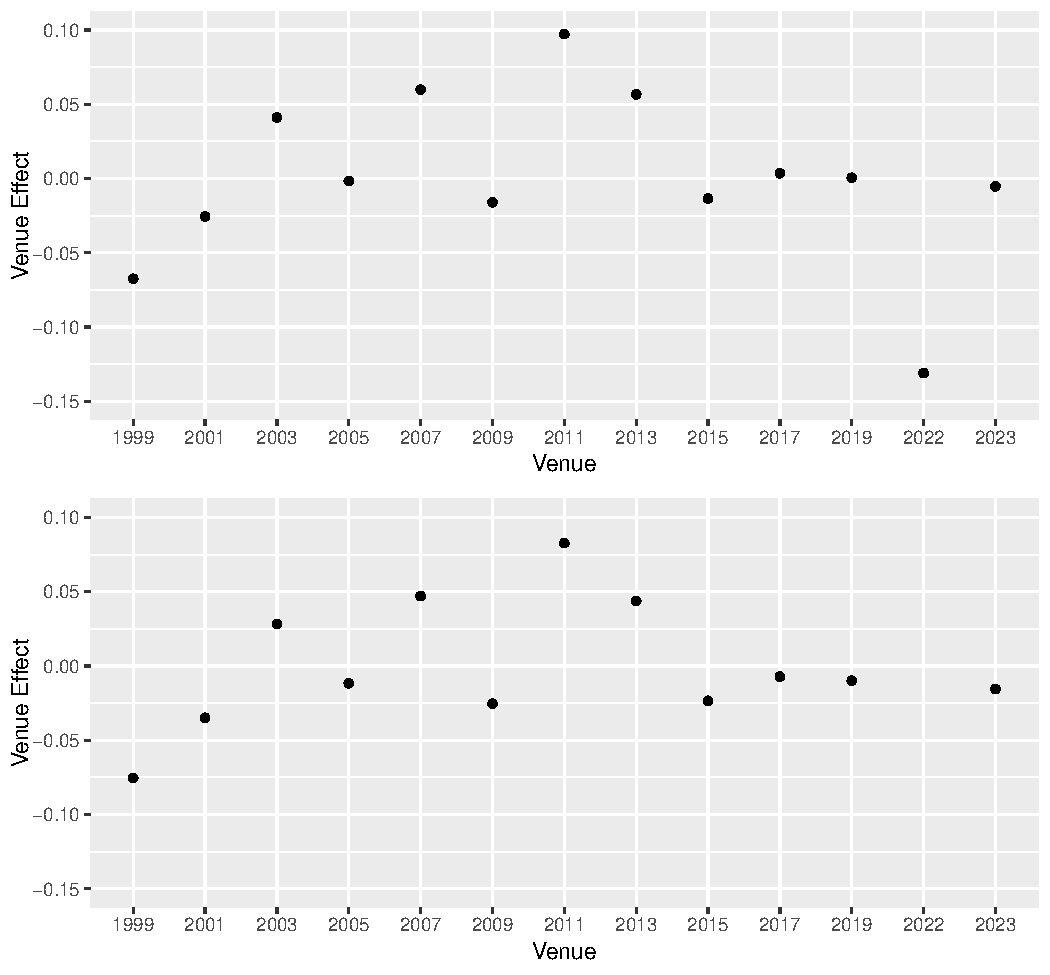
\includegraphics{ComparisonOfVenueEffects}
  \caption{The venue effects from 1999 to 2023 estimated from the GLMM for the
    data including 2022 (top) and excluding 2022 (bottom).}
  \label{fig:VenueEffects}
\end{figure}


Figure~\ref{fig:VenueEffects} further illustrates the venue effect from 1999 to
2023 based on the full GLMM both with and without 2022.  The temporal patterns
of the two sets of effects look very similar, except that the positive effects
estimated with 2022 included have higher magnitude than those estimated without
2022, which compensates the negative effect of the 2022 with a large magnitude.
Both plots agree to some extent with the pattern of the centers of the boxplots in
Figure~\ref{fig:Boxplot}. The mismatch is due to the venue effect, which has a
higher standard deviation than the venue effect. 
\eds{I do not understand what is meant by the previous sentence.}
The venue effect for 2022 is
lower than that for any other year, but may not be as extreme as one would
think considering the history of reaction times going back to 1999.


\begin{table}
  \centering
  \caption{Probabilities of observing reaction times less than threshold 0.08,
  0.09, and 0.10 seconds based on the two effect model.}
  \begin{tabular}{c c c c} 
   \toprule
   Data Set & Threshold 0.08 & Threshold 0.09 & Threshold 0.10  \\ 
   \midrule
   Excluding 2022 & $3.35\cdot10^{-5}$ & $4.45\cdot10^{-4}$ &  $3.54\cdot10^{-3}$  \\ 
   Including 2022 & $4.20\cdot10^{-5}$ & $5.70\cdot10^{-4}$ & $4.34\cdot10^{-3}$ \\
   \bottomrule
  \end{tabular}
  \label{tab:Sim_probability}
\end{table}

The GLMM with both venue and heat random effects helps us to assess how extreme
a reaction time below a given threshold is. The probability of observing a reaction
time below a threshold, assuming no intentional false starts, can be
approximated by generating a large number of realizations from the fitted
GLMM. We used 10 millions realizations in the analysis. 
Table~\ref{tab:Sim_probability} summarizes the estimated probabilities of
observing a reaction time below 0.08, 0.09, and 0.10 seconds under two different
scenarios: one excluding and the other including data from 2022. Apparently,
excluding 2022 lowered the probability of observing a fast reaction time, but
the difference is not big in magnitude. For example, the probability for
seeing a reaction time below 0.10 seconds changes from $3.54\cdot 10^{-3}$ to
$4.20\cdot 10^{-3}$ when 2022 is included. These values correspond to roughly one in
every 230 starts and 283 starts, respectively. The table shows that changing the
reaction time barrier from 0.1 seconds to 0.08 seconds drastically reduces the
chance of observing a reaction time below the barrier, from one in roughly every
283 starts to one in every 29851 starts using data with 2022 included. The
results substantiates the recommendations by \citet{komi2009iaaf}.


\begin{table}
  \centering
  \caption{Suggested reaction time barriers based on tail probabilities.}
  \begin{tabular}{c c c} 
   \toprule
   Data Set & Tail probability  $10^{-3}$ & Tail probability $10^{-4}$ \\ 
   \midrule
   Excluding 2022 & $0.094$ & $0.084$ \\ 
   Including 2022 & $0.092$ & $0.083$ \\
   \bottomrule
  \end{tabular}
  \label{tab:Sim_time}
\end{table}


Utilizing the same model, we can subtly shift our interpretation to determine a
suitable reaction time barrier based on the probability of observing a time
below said barrier. Including 2022 data, a reaction time barrier of 0.092
seconds is warranted to maintain a 0.1\% chance of observing an illicitly fast
reaction time, as delineated in Table~\ref{tab:Sim_time}. This calculation can
be replicated for various probability levels; for instance, a probability of
0.0001 (equating to one disqualification per 10,000 starts) necessitates a
reaction time barrier of 0.083 seconds. The exclusion of 2022 data, which
inherently lowers the probability of observing a swift reaction time, mandates a
less lenient reaction time barrier when calculated based on probability, albeit
without a substantial difference in magnitude.


\section{Discussion}\label{sec:concludingremarks}


We did not consider data from the women's 100 meter hurdle in the analysis.
In addition to the concerns over reaction time differences in men and
women, exploratory analysis showed that 2022 women were at best only
slightly faster relative to other championships going back to 2003.
Likewise, the rank-based comparisons resulted in p-values
that were not drastically significant after adjusting for multiple tests.
The lack of evidence from the women's data makes it 
harder to conclude that the sensors used at the 2022 championships were faulty, 
although it is unknown if the sensors for the men's 110 meter hurdle and women's
100 meter hurdle were the same. On the other hand, this may be related to 
another debated question regarding whether the reaction time barrier should be 
the same for men and women.


The uniformity of the reaction time barrier for both men and women is
perplexing, especially in light of numerous studies that suggest a divergence in
their respective reaction times \citep[e.g.,][]{lipps2011implications,
  babicc2009reaction, panoutsakopoulos2020gender}. These authors posit that
World Athletics may be overlooking inherent gender differences by establishing
an equal reaction time barrier. If gender disparities do exist and 0.1 seconds
is deemed a fair threshold for women, it logically follows that the same cannot
be deemed fair for men, given that the probability of observing sub-0.1-second
reaction times would be inherently higher. \citet{brosnan2017effects} propounds
the adoption of gender-specific reaction time barriers, a stance that appears
logical when considering biological distinctions in reaction times between
genders.


This paper aspires to offer a statistical lens through which to examine Allen's
disqualification at the 2022 World Track and Field Championships, rather than
delivering a conclusive judgment regarding potential equipment malfunction. Our
findings reveal that athletes' reaction times at the event were, in general,
faster than those recorded at other competitions, with
Table~\ref{tab:Clusrankresults} presenting multiple significant p-values that
highlight disparities in average reaction times between the 2022 Championship
and other competitions. Further, our GLMM results indicate that a reaction time
of 0.1 seconds may not be as exceptional as commonly believed. According to the
probabilities in Table~\ref{tab:Sim_time}, World Athletics might contemplate
adjusting the disqualification barrier to 0.8 seconds, thereby enabling athletes
like Allen to react more swiftly without the apprehension of
disqualification. In summary, while the results designate 2022 as an anomalous
year, Allen's time, despite resulting in disqualification, may not be
categorically extreme.


\section*{Supplementary Material}
The data and R code used for the analysis are available in a compressed file for
ease of reproducibility.

\bibliographystyle{chicago}
\bibliography{citations}


\end{document}
